\chapter{Discussions} \label{ch:discussions}

    \section{Overview}
    
    \section{Ways to further improve}
        \subsection{Disentanglement metric}
            There are some thoughts we wish to discuss on the disentanglement metric used in this project. By working with the metric proposed by \cite{kim2018disentangling}, we really found the computational simplicity really helpful, especially in saving time to run them. Also, the fact that the metric used a parameter-free deterministic classifier helped to have more consistent and robust standard of criteria for comparing models over various settings including the change of the size of the latent space.
            
            However, we did make a simple observation which could potentially help to significantly improve the sensitivity of the metric. Recall(as explained in section \ref{subsec:metric_kim}), that the metric looks for the argmin across the normalised latent dimensions of the encoded values of images generated with a single generative factor fixed for calculating the disentanglement score. The limitation with this approach is that this results in the loss of information of \textit{how small} the dimension with the argmin is. Consider two scenarios. The first scenario is when the model has ideally and perfectly made a disentangled representation of the input space. In this case, the normalised variance with the argmin will be zero. The second scenario is when the model learned a poor disentangled representation but has managed to disentangle enough for there to be a one-to-one correspondence between argmin dimensions and the generative factors. In this case, according to the metric, the model could potentially, though unlikely, achieve a high disentanglement score, because the metric does not care \textit{how small} the minimum normalised variance is as long as it is \textit{relatively} the smallest. Although in practice, getting a high score is still unlikely because if the model's latent encodings are strongly entangled, the argmin of the generated samples will highly be inconsistent across samples which leads to a lower disentanglement score. However, it seems like a waste of valuable information to not take into account how small the lowest variance was.
            
            One way we could make use of the variances across the dimensions is by adding a weight to the votes which takes into account of the variances. For example, consider:
               \[w = \frac{\left|\left(\sum_{d=1}^D \sigma_d \right) - \sigma_{min}\right|}{\sum_{d=1}^D \sigma_d}\]
            With this weight $w$, the vote would weigh maximal if the relative variance at argmin is close to zero, and the weight of the vote would be minimal if the relative variance is close to the total variance. This can potentially provide more sensitive disentanglement metric which takes into account of \textit{how small} the variance is at argmin instead of just taking argmin into account.
            
        \subsection{Loss function}
            Theoretically, as discussed in \ref{subsec:beta_reasoning}, it made much sense to let the loss function include a \textit{weighted} KL-divergence term in order to control how efficiently we require the model to encode the images. However, the changes of the weight value $\beta$ did not always show recognisable differences in the experiments from this project. There were very specific settings in which the $\beta$ value did make a clear difference, but in many settings, there was not a big improvement as one hoped for.
            
            More recent paper by \cite{burgess2018understanding} suggested some further changes to the loss function which could improve the performance. Let us recall what the $\beta$ value is encouraging the model to do. If $\beta=0$, i.e. when there is no KL divergence, then the latent distributions will tend to be very sharp Gaussians, i.e. with very small variances, with the mean values heavily varying depending on the input values. Larger $\beta$ values enforce the Gaussians to have wider variances and the mean values to not vary too much by encouraging them to be close to zero. In the information bottleneck perspective(as discussed in section \ref{subsec:beta_reasoning}), increasing the $\beta$ decreases the information bottleneck by encouraging the KL divergence to be zero. Now it isn't that we actually want the distributions' KL divergence to be actually \textit{zero}. Instead, by pushing the KL divergence towards zero by the appropriate amount, controlled by $\beta$, we want the KL divergence to arrive at an optimal value which is not too big, for it not to learn anything, nor too small, for it to learn in entangled manner. However, if what we what we are aiming for is encouraging the model to have some specific value of an optimum KL divergence, may be adjusting the pressure for the KL divergence to stay close to zero is not the most efficient way. This is exactly what the new loss function by \cite{burgess2018understanding} aims to address:
            
            \begin{equation}
                \text{Loss\textsubscript{$\beta$-VAE2}} = \mathbb{E}_{q_{\bm{\theta_x}}(\bm{z}|\bm{x})} \left[\log p(\bm{x} | \bm{z}) \right] + \textcolor{red}{\gamma} \textcolor{red}{|} KL\left[q_{\bm{\theta_x}}(\bm{z}|\bm{x}) || p(\bm{z})\right] \textcolor{red}{-C} \textcolor{red}{|}
            \end{equation}
            
            Although the equation above may look similar to the original $\beta$-VAE loss function, there is a subtle difference in the objective it is trying to achieve. The new $\gamma$ term essentially plays the same role as the previous $\beta$ term: it acts as a weight to this newly transformed KL divergence. The new $C$ term is what controls the \textit{capacity} of the information bottleneck. In the original $\beta$-VAE equation, the capacity term was zero and so the weight parameter was always directing the model towards a zero KL divergence. However, now in this new equation, we can specify what value of the KL divergence we want the model to aim for. Furthermore, \cite{burgess2018understanding} made the capacity term vary over time by linearly increasing it from a preset range. This was motivated by the observation that different features were learnt at different values of capacity as shown by the figure below:
            
            \begin{figure}[H]
                \centering
                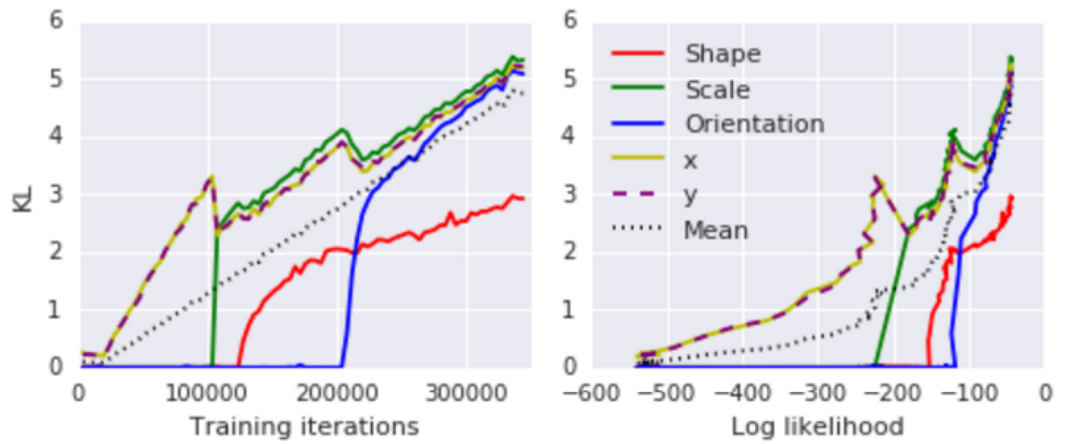
\includegraphics[width=0.6\textwidth]{imgs/features_capacity.png}
                \caption{Figure from \cite{burgess2018understanding}. Left graph: the y-axis is the KL divergence(in nats) and the x-axis is the number of training iterations. The graphs show the KL divergence of the dimension which correspond to representing a specific generative feature. The once a dimension learns to represent a generative feature, the KL divergence increases as the distribution strays away from the standard Gaussian. The The grey dotted line is the mean value of the KL divergence which also represents the value of the increasing capacity $C$ over the iterations. At different values of capacity given, different generative features were learnt in the order depending on the KL divergence capacity required to learn. Right graph: same graph as the left graph except across the log reconstruction likelihood instead of the training iterations.}
                \label{fig:features_capacity}
            \end{figure}
            
            Making the loss a function of the reconstruction error, the weighted KL divergence, as well as the the target capacity and the training iteration seems like a step forward in improving the performance. As an extension for this project, we wish to experiment with this new loss function to test whether or not this makes a significant performance improvement over the original $\beta$-VAE.
            
            One other factor which could be worth considering is to put constraints on the KL divergence across different dimensions \textit{separately}. For example, as we can see from the figure \ref{fig:features_capacity} above, different features are learnt across different dimensions at different available capacities. Perhaps we could experiment what happens if we start with varied KL divergence capacity targets across the latent dimensions from the start. Another way we could use separate KL divergence weights across separate dimensions is to vary the weight according to how much KL divergence each dimension has at a given iteration. Increase in KL dimension in a given dimension is an indirect indication of it having learnt a generative feature. At this point, we probably want to increase the capacity across other unlearnt dimensions to allow it to learn features which require higher capacity. However, if we increase the capacity across the whole, the learnt dimension could use this capacity to unnecessarily learn more inefficient, entangled representations to increase the reconstruction accuracy. To prevent this, once a KL divergence in one dimension significantly increases and settles, we could set this KL divergence value to be the capacity target for this dimension only and give it an increasingly higher weight so that this dimension "stops learning" to give other dimensions the opportunity to learn other features by increasing the capacity across other dimensions.